\begin{surferPage}[216 Singulariteiten]{Oppervlakken met veel re\"ele singulariteiten}
    Zoals reeds gezegd is het maximum aantal singulariteiten
    $\mu(7)$ op een oppervlak van graad $7$ niet gekend.
   We kennen enkel een onder- en bovengrens: $99\leqslant \mu(7) \leqslant 104$. 


    Het hoeft dus niet te verbazen dat voor algemene graad $d$ nog veel minder geweten is. 

    Sonja Breske, Oliver Labs en Duco van~Straten zijn er toch in geslaagd om een constructie van S.V.\ Chmutov zo aan te passen dat het huidige maximale aantal singulariere punten ook bereikt wordt door oppervlakken met re\"ele singulariteiten. 
    Voorlopig weten we dat:
    \[0,41\bar{6}d^3 \lessapprox \mu(d) \lessapprox 0.44\bar{4} d^3.\]
     Als we langs de bovenkant kijken, zien we een verband tussen de symmetrie van het oppervlak en het maximaal aantal zwarte vlakken in een verzameling snijdende rechten:
    \begin{center}
      \begin{tabular}{c@{\qquad}c}
        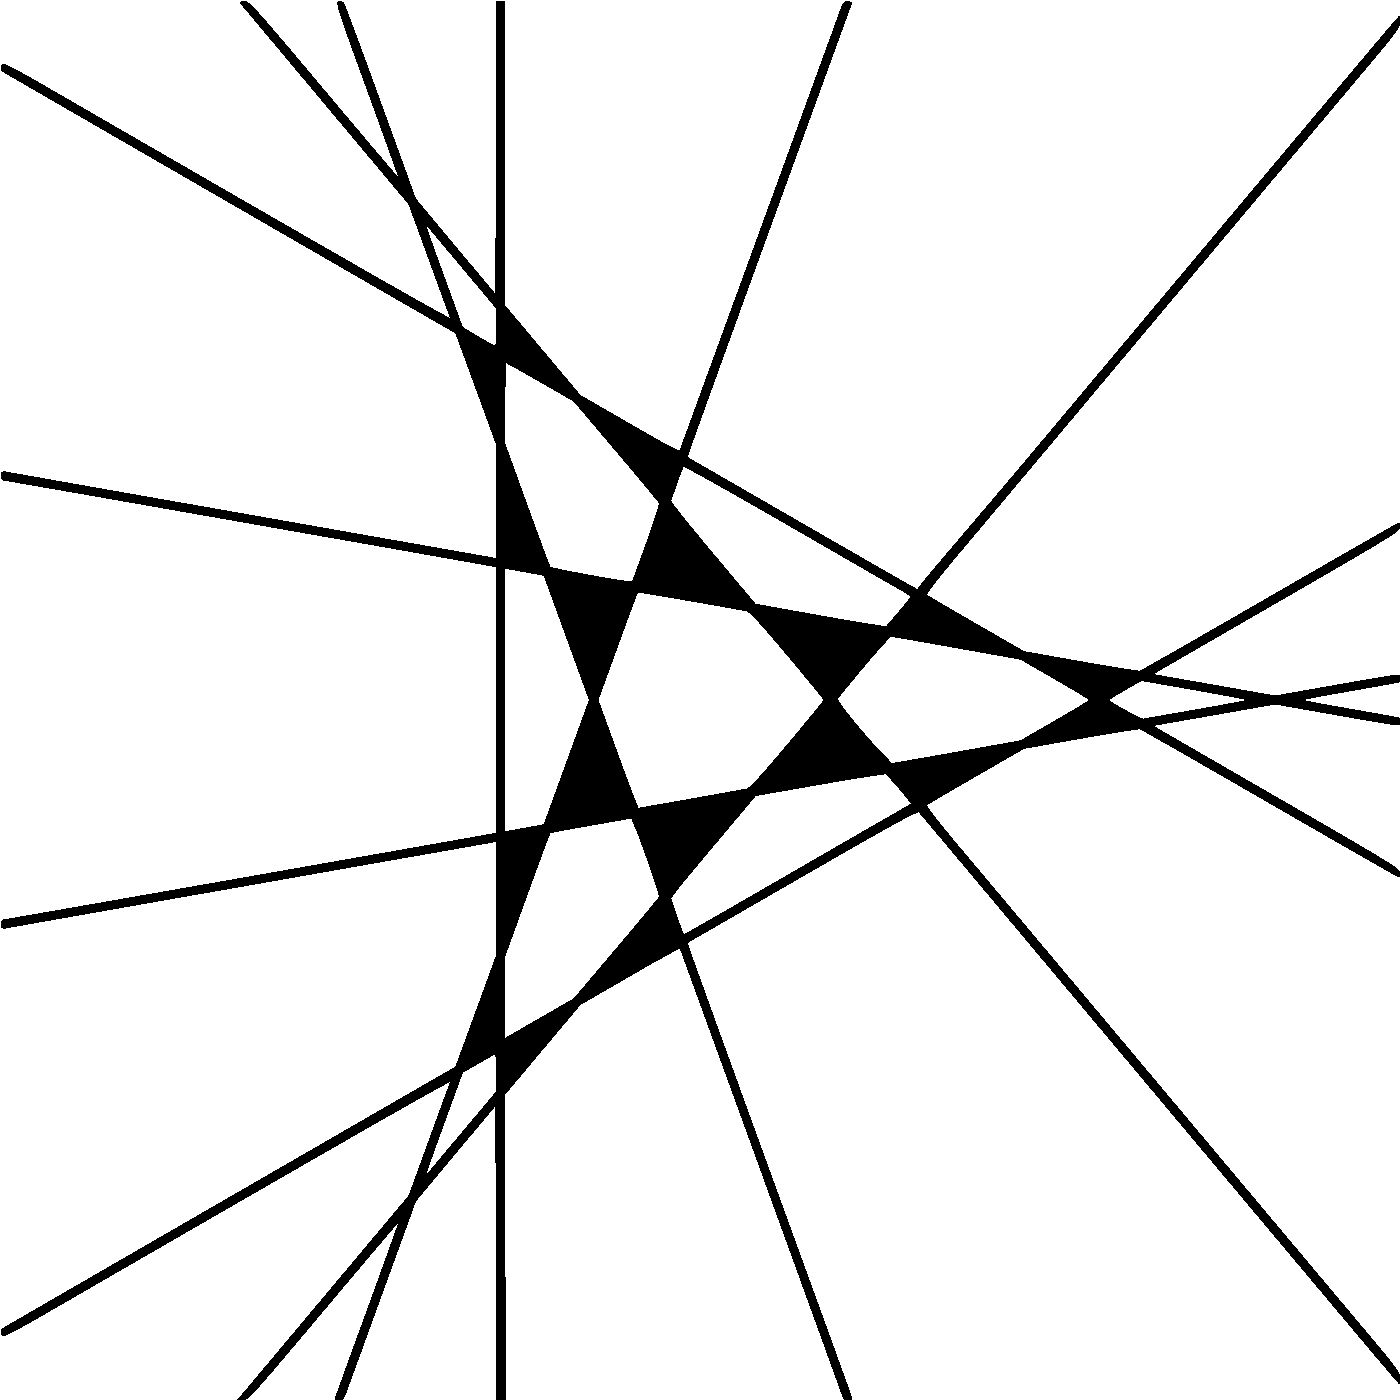
\includegraphics[height=1.5cm]{./../../common/images/vielesing.pdf}
        &
        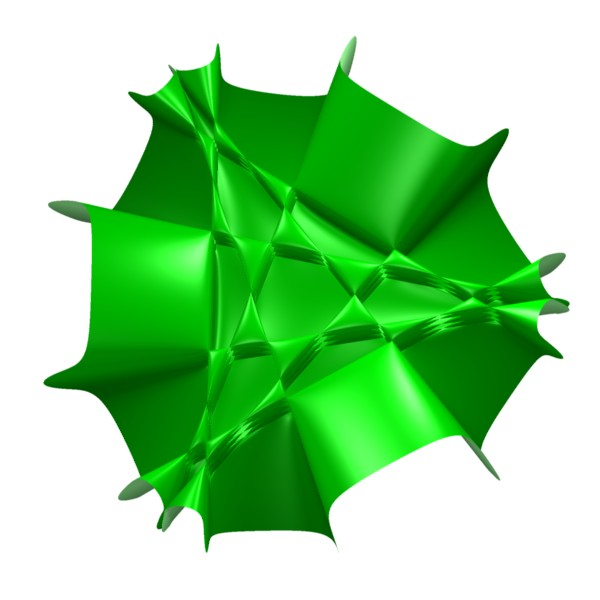
\includegraphics[height=1.5cm]{./../../common/images/p9surface_von_oben}
      \end{tabular}
    \end{center}
\end{surferPage}
